% === T15 - Introducción a los Sistemas Operativos ===
% David Alejandro Gonzalez Marquez
% fokerman@gmail.com
% https://github.com/fokerman/computingSystemsCourse

\documentclass[aspectratio=169]{beamer}
\usepackage{../packages}

\title{\Huge Introducción a los Sistemas Operativos}
\author{David Alejandro González Márquez}
\institute{}

\date{}

\begin{document}

\begin{frame}[plain]
    \titlepage
    \begin{textblock}{100}(30,80)
    \begin{tcolorbox}[size=small,width=\textwidth,colback={gray!30},title={}]
    \begin{center}
     \scriptsize Clase disponible en: \url{https://github.com/fokerman/computingSystemsCourse}
    \end{center}
    \end{tcolorbox}
    \end{textblock}
%     \begin{textblock}{140}(10,70)
%     \textcolor{rojo}{
%     \textbf{Atención}: La clase será grabada por el anfitrión para su posterior y eventual uso académico dentro de nuestra institución. Su participación en la clase implica brindar su consentimiento para participar en la grabación, aunque pueden mantener su video apagado.}
%     \end{textblock}
\end{frame}

\begin{frame}{¿Qué Sistemas Operativos conocen?}
    \begin{textblock}{80}(5,15)
        \scriptsize
        \begin{itemize}
        \item[] \textbf{Microsoft}
        \begin{itemize} \scriptsize 
            \item MS-DOS
            \item Windows
            \item Windows Phone
        \end{itemize}    
        \item[] \textbf{Sun Microsystems}
        \begin{itemize} \scriptsize 
            \item SunOS
        \end{itemize}    
        \item[] \textbf{Oracle}
        \begin{itemize} \scriptsize 
            \item Solaris
        \end{itemize}
        \item[] \textbf{NeXT}
        \begin{itemize} \scriptsize 
            \item NeXTSTEP
        \end{itemize}
        \item[] \textbf{Apple Macintosh}
        \begin{itemize} \scriptsize 
            \item Mac OS
            \item Darwin
            \item Newton OS
            \item iOS
        \end{itemize}
        \item[] \textbf{BlackBerry}
        \begin{itemize} \scriptsize 
            \item BlackBerry OS
        \end{itemize}
        \end{itemize}
    \end{textblock}
    \begin{textblock}{80}(40,15)
        \scriptsize
        \begin{itemize}
        \item[] \textbf{Symbian Ltd.}
        \begin{itemize} \scriptsize 
            \item Symbian
        \end{itemize}
        \item[] \textbf{Berkeley Software Distribution (BSD)}
        \begin{itemize} \scriptsize 
            \item BSD
            \item Free BSD
        \end{itemize}
        \item[] \textbf{GNU/Linux}
        \begin{itemize} \scriptsize 
            \item Debian
            \item Ubuntu
            \item Fedora
            \item RedHat
            \item Kali Linux
            \item Raspberry Pi OS
            \item OpenWRT
            \item Google - Android 
            \item Google Chrome OS
        \end{itemize}
        \end{itemize}
    \end{textblock}
    \begin{textblock}{80}(50,78)
    \scriptsize
    Para ver ejemplos de estos\\
    sistemas operativos:\\
    \url{https://copy.sh/v86/}
    \end{textblock}
    % Figuras    
    \begin{textblock}{80}(93,2)  
    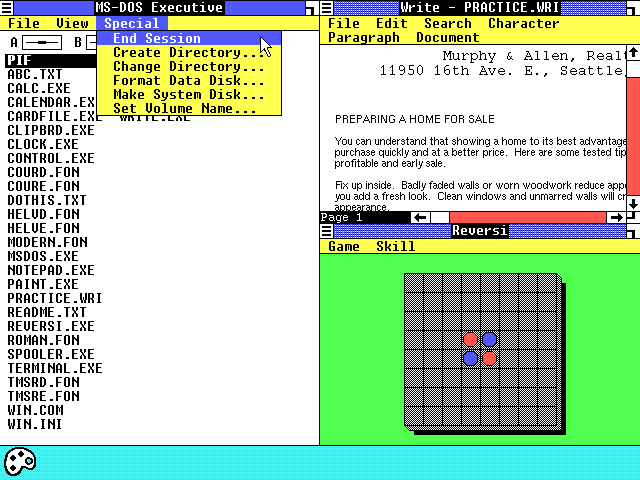
\includegraphics[height=2.2cm]{img/Microsoft_Windows_1.0_1985.png} \hspace{0.1cm}
    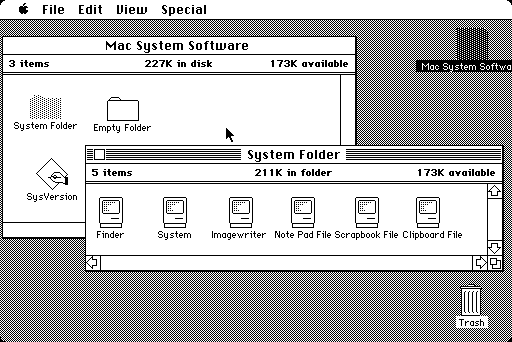
\includegraphics[height=2.2cm]{img/Apple_Macintosh_Desktop_1990.png} 
    \end{textblock}
    \begin{textblock}{100}(93,25)
    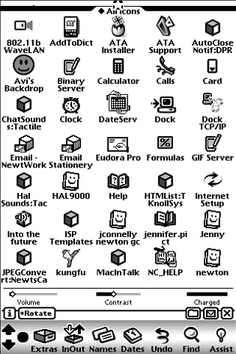
\includegraphics[height=1.93cm]{img/Apple_NewtonOS_1993.png} \hspace{0.01cm}
    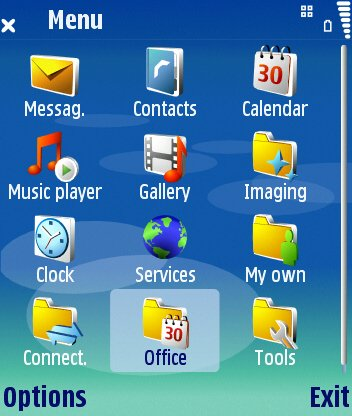
\includegraphics[height=1.93cm]{img/n80_2005.jpg}
    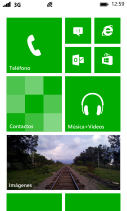
\includegraphics[height=1.93cm]{img/Windows_Phone_2010.pdf}
    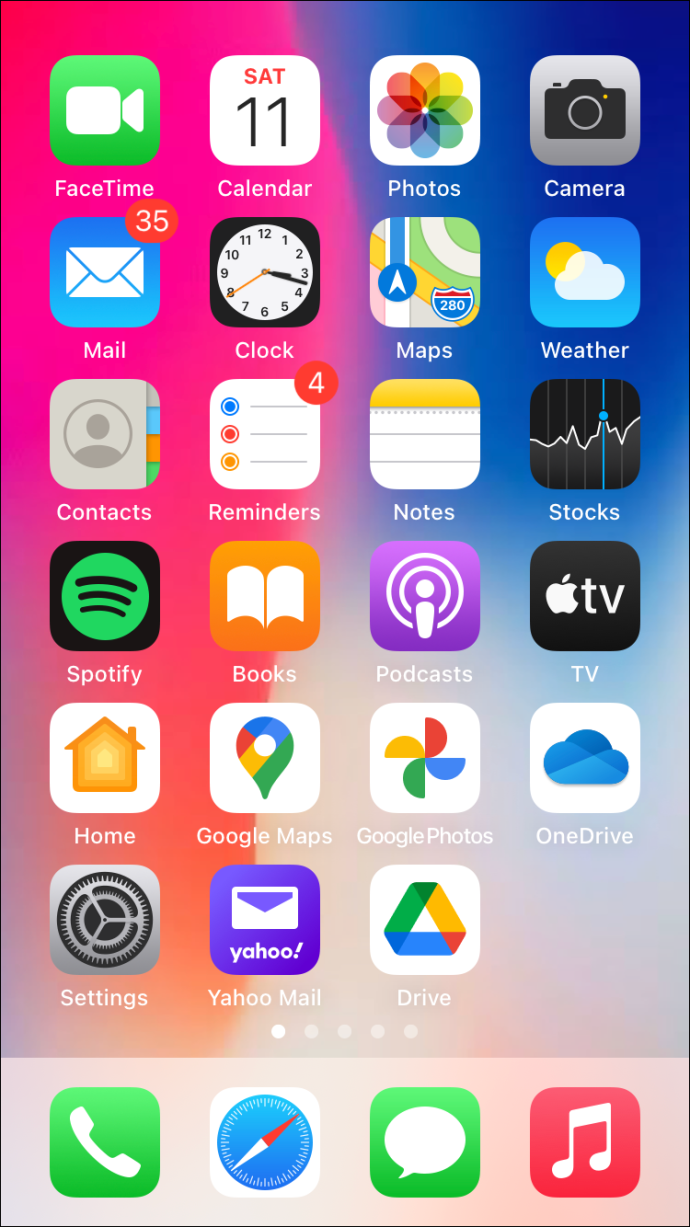
\includegraphics[height=1.93cm]{img/iOS_2020.png}
    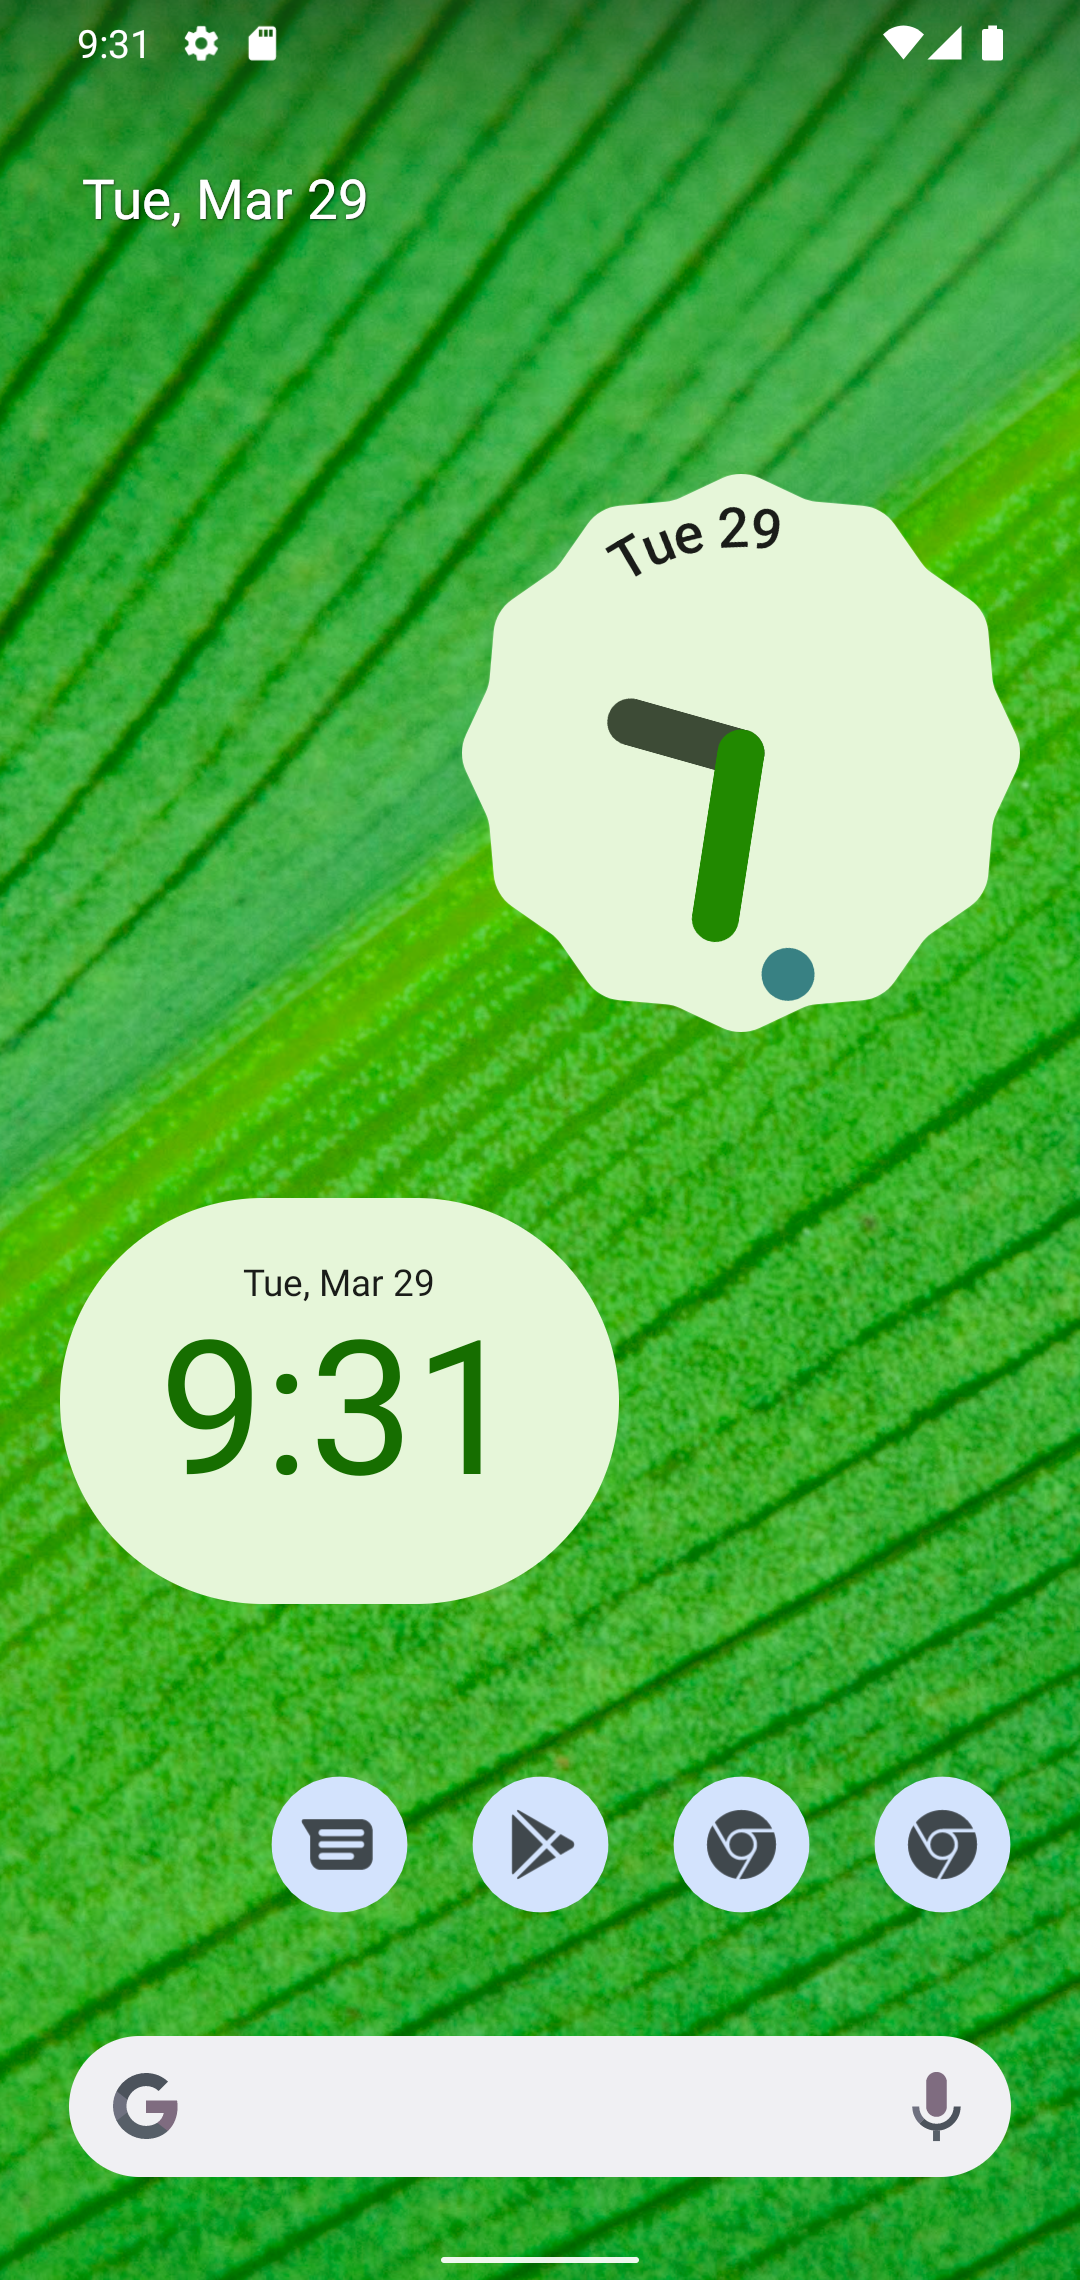
\includegraphics[height=1.93cm]{img/Android_12_2021.png}
    \end{textblock}
    \begin{textblock}{80}(93,45.5) 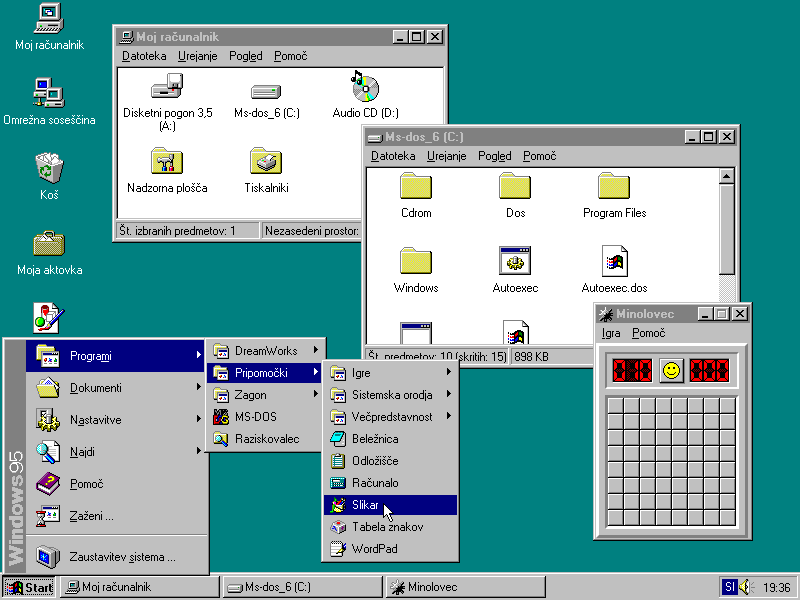
\includegraphics[width=3cm]{img/Windows_1995.png} \end{textblock}
    \begin{textblock}{80}(126,45.5) 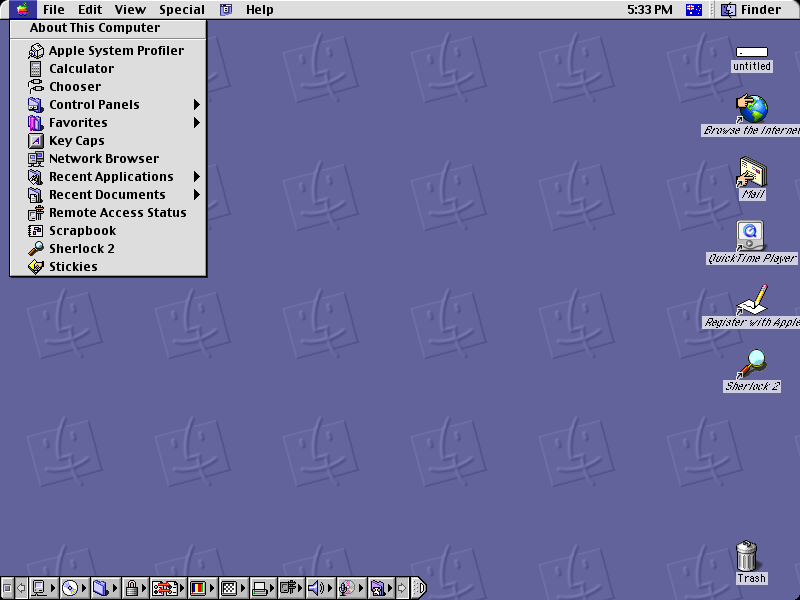
\includegraphics[width=3cm]{img/Mac_OS_9.0.4_1999.png} \end{textblock}
    \begin{textblock}{80}(93,69) 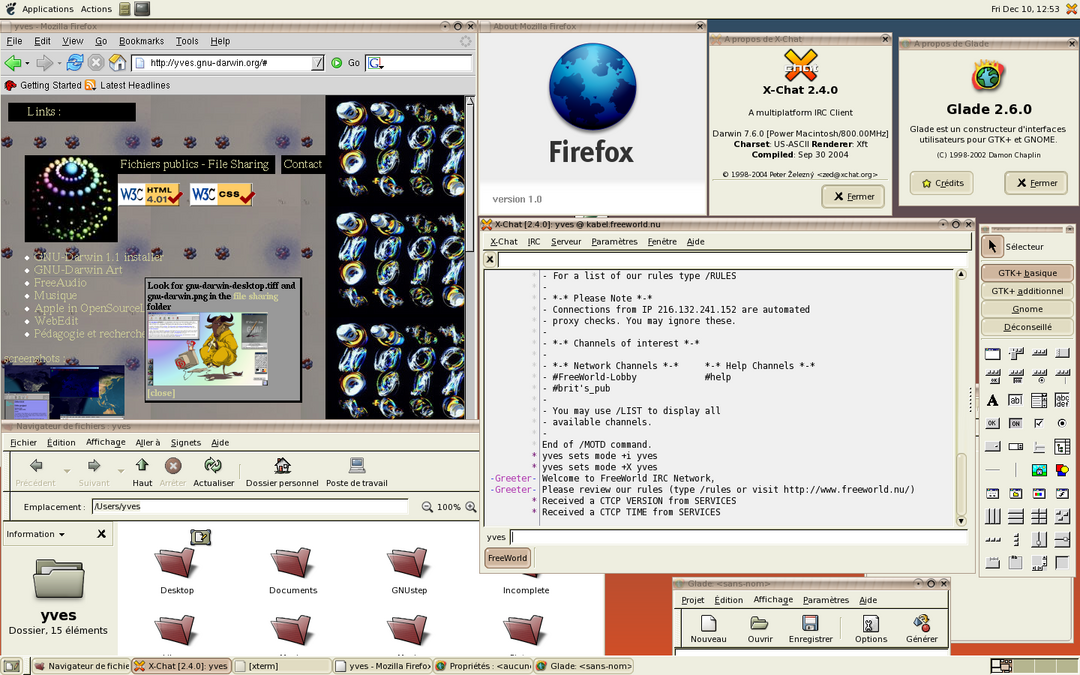
\includegraphics[width=3cm]{img/Darwin_GNOME_2_2004.png} \end{textblock}
    \begin{textblock}{80}(126,69) 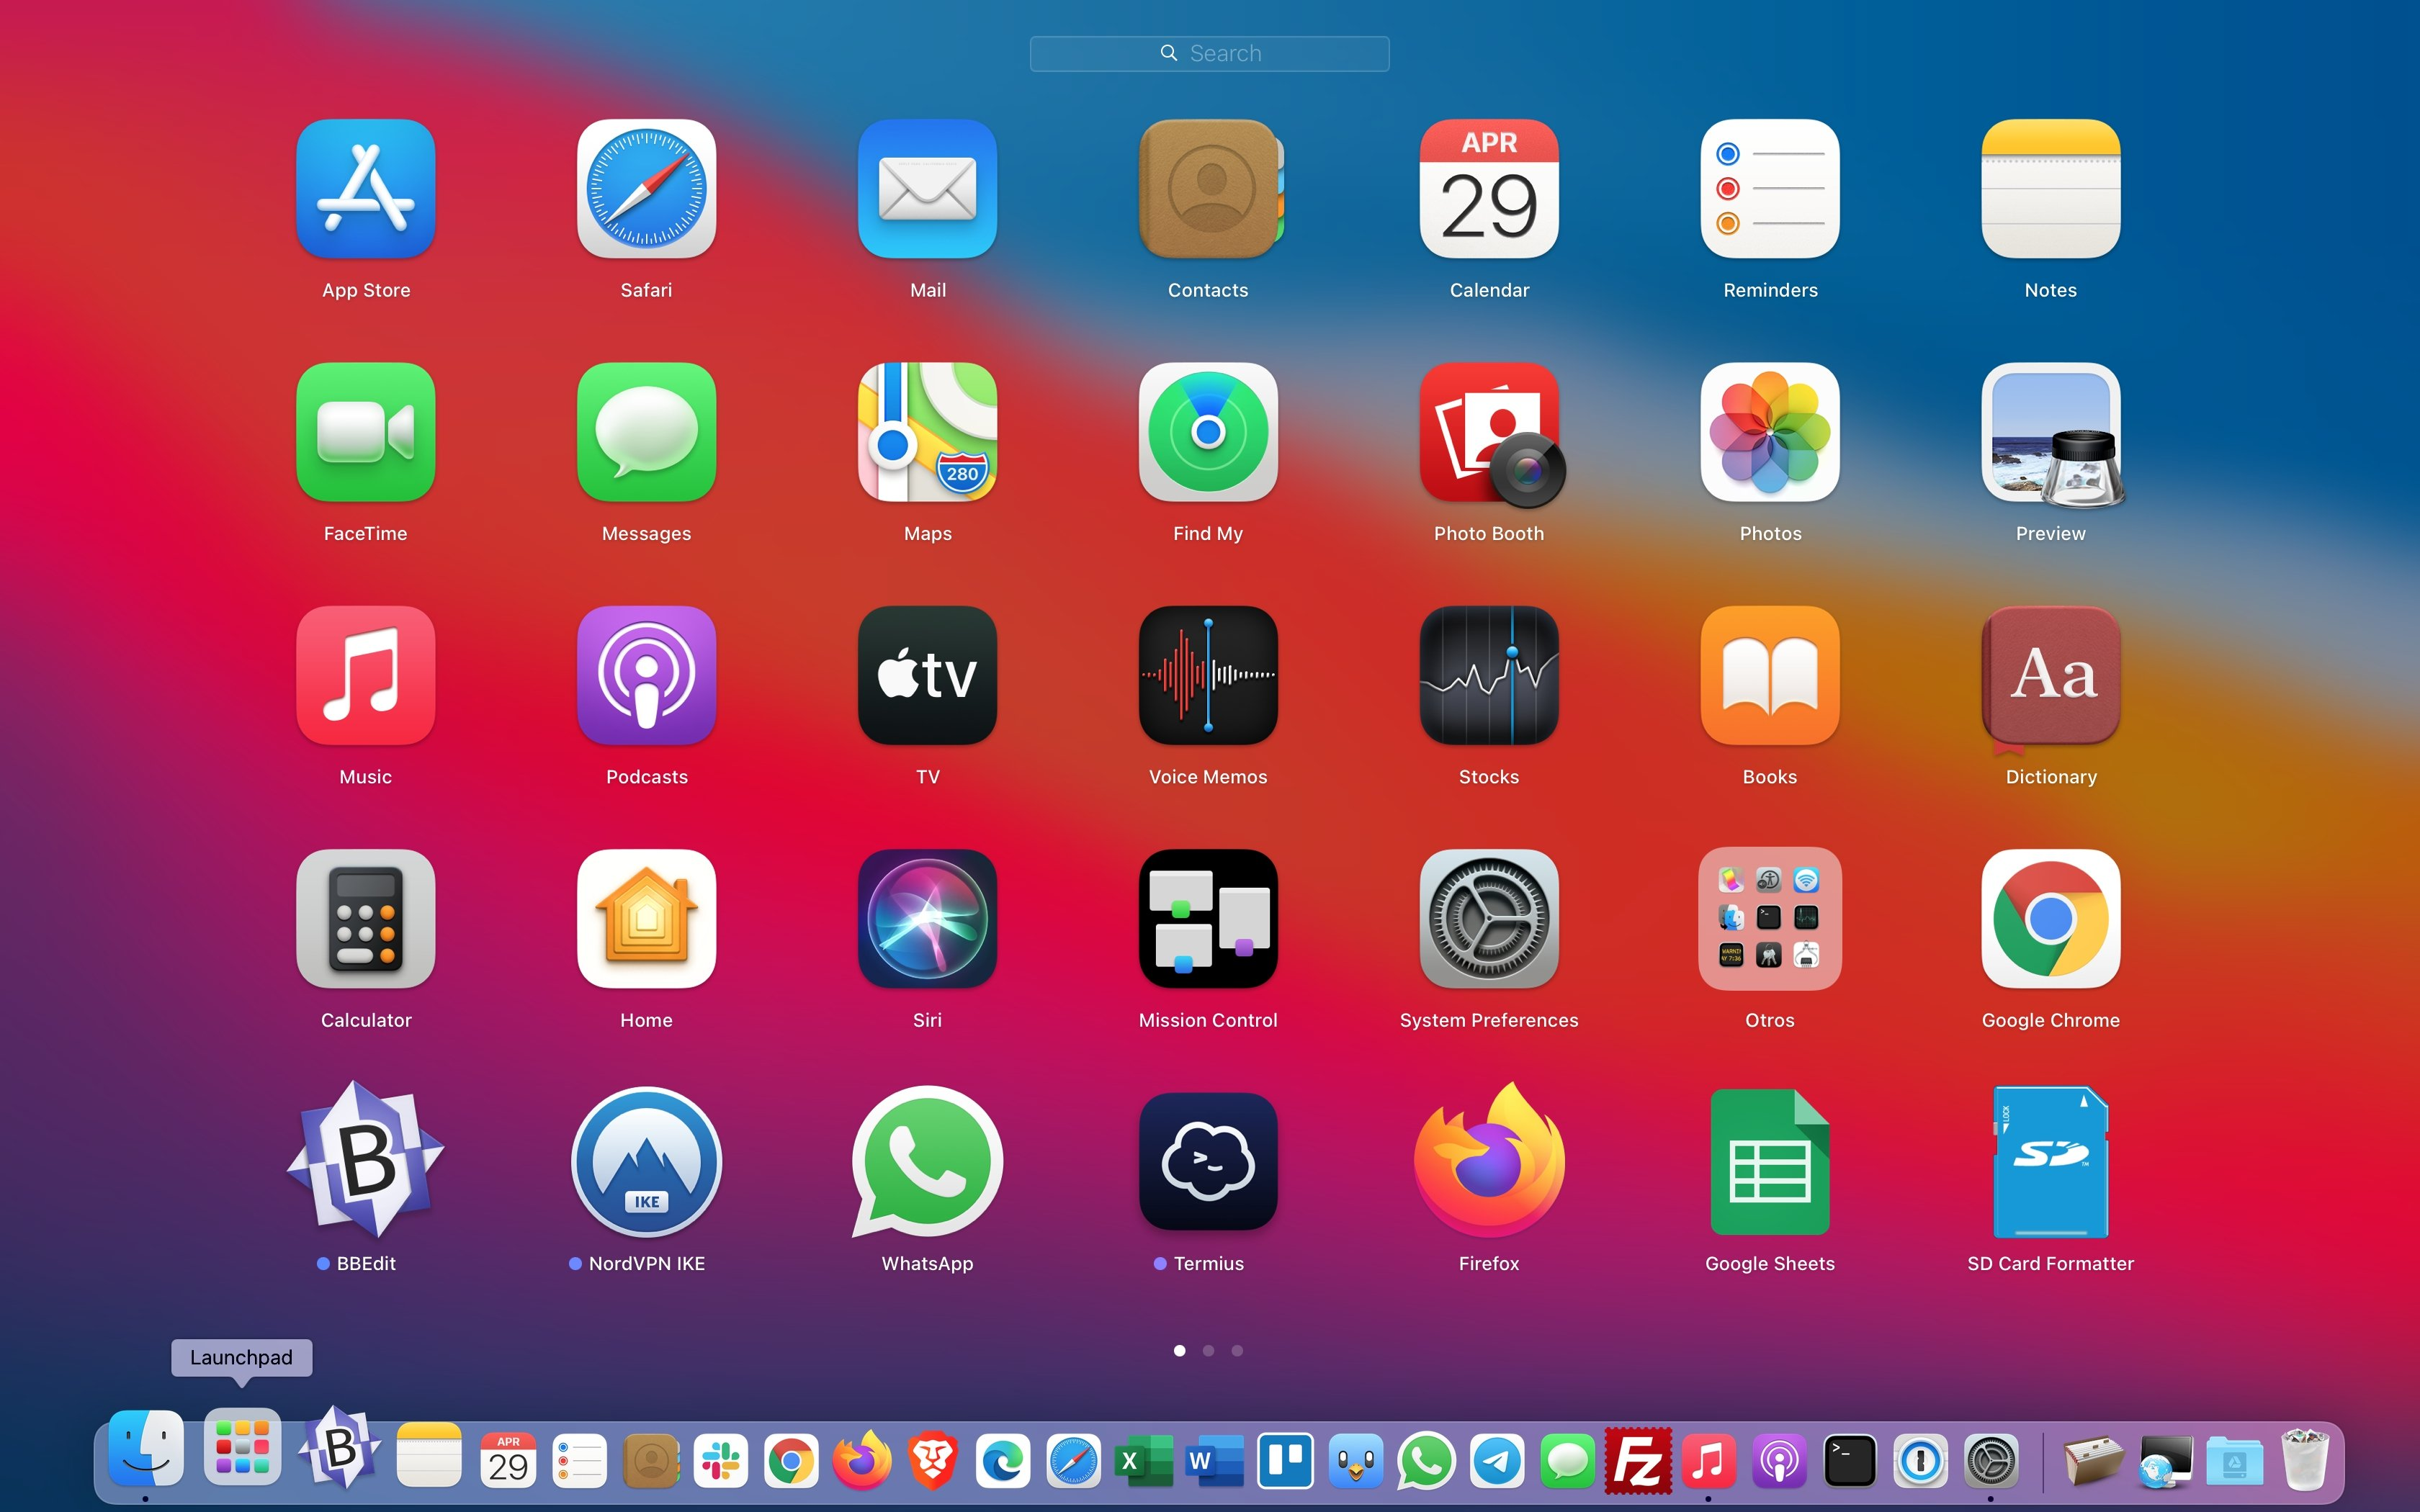
\includegraphics[width=3cm]{img/macos-10_2020.jpg} \end{textblock}
    % Años
    \begin{textblock}{80}(100,20) 1985 \hspace{2.3cm} 1990 \end{textblock}
    \begin{textblock}{180}(96,40) 1993 \hspace{0.7cm} 2005 \end{textblock}
    \begin{textblock}{180}(126,26) 2010 \hspace{0.3cm} 2020 \hspace{0.2cm} 2021 \end{textblock}
    \begin{textblock}{80}(114,46.5) 1995 \end{textblock}
    \begin{textblock}{80}(144,47.5) 1999 \end{textblock}
    \begin{textblock}{80}(114,80) 2004 \end{textblock}
    \begin{textblock}{80}(147,83) 2020 \end{textblock}
\end{frame}

\begin{frame}[plain]
    \begin{textblock}{80}(5,12)
    \textcolor{naranjauca}{\Large Línea de tiempo de Unix}
    \end{textblock}
    \begin{textblock}{80}(25,5)
    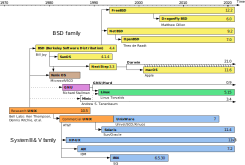
\includegraphics[scale=0.50]{img/unix_timeline_en.pdf}
    \end{textblock}
\end{frame}

\begin{frame}{Sistemas Operativos}
    \vspace{0.7cm}
    \begin{tcolorbox}[width=\textwidth,colback={verdeuca!30},title={}]
    El \textbf{sistema operativo} es un administrador de recursos de Hardware.
    Su responsabilidad fundamental es la designación de recursos de hardware para cada programa a ejecutar.
    \end{tcolorbox}
    \small
    \bigskip
    \pause
    Es una \textcolor{verdeuca}{\textbf{compleja pieza de Software}} diseñada para soportar distintos tipos de comportamientos y usos.\\
    Desde computadoras personales o smartphones, hasta dispositivos embebidos como routers.\\
    \bigskip
    \pause
    Las primeras computadoras no requerian de un sistema operativo como hoy lo conocemos.\\
    Eran en cambio, programas que facilitaban \textcolor{verdeuca}{\textbf{la carga de los programas}} dentro del sistema.\\
    \bigskip
    El avance de la computación hizo surgir la necesidad de un pograma que opere como \textcolor{verdeuca}{\textbf{mediador}} entre los recursos de hardware y los programas de usuario.
\end{frame}

\begin{frame}[t]{Punto de vista del usuario}
    Nos provee una interfaz para poder \textcolor{verdeuca}{\textbf{interactuar}} con el sistema
    \begin{textblock}{50}(15,27)
    \normalsize \textbf{GUI} (\emph{graphical user interface)}\\
    \small Permite manipular ventanas y menúes mediante el mouse y teclado.
    \end{textblock}
    \begin{textblock}{50}(15,60)
    \normalsize \textbf{CLI} (\emph{command-line interface)}\\
    \small Permite escribir comandos de texto mendiante el teclado en una consola.
    \end{textblock}
    \begin{textblock}{50}(75,22)
    \includegraphics[scale=0.35]{img/cli_gui-layer1.pdf}
    \end{textblock}
    \begin{textblock}{50}(75,55)
    \includegraphics[scale=0.35]{img/cli_gui-layer2.pdf}
    \end{textblock}
\end{frame}

\begin{frame}{Punto de vista del usuario}
    \begin{textblock}{80}(5,20)
    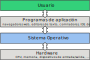
\includegraphics[scale=0.8]{img/vista_abstracta_componentes.pdf}
    \end{textblock}
    \begin{textblock}{70}(80,10)
    \small
    \begin{itemize}
    \item<1->[] Los programas de usuario se comunican con el Sistema Operativo para acceder a \textbf{recursos}.
    \item<1->[] \textcolor{naranjauca}{¿Cúales recursos requieren los programas?}
    \item[] 
    \item<2->[] El Sistema Operativo provee una \textbf{interfaz} para acceder al hardware.
    \item<2->[] \textcolor{naranjauca}{¿Cúal es y cómo funciona esta interfaz?}
    \item[] 
    \item<3->[] Para el usuario, el programa tiene todos los recursos que necesita, cuando en realidad los está \textbf{compartiendo}.
    \item<3->[] \textcolor{naranjauca}{¿Cómo se comparte un recurso?}
    \end{itemize}
    \end{textblock}
\end{frame}

\begin{frame}{Punto de vista del usuario}
    \begin{textblock}{80}(5,20)
    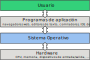
\includegraphics[scale=0.8]{img/vista_abstracta_componentes.pdf}
    \end{textblock}
    \begin{textblock}{72}(80,10)
    \small
    \begin{itemize}
    \item<1->[] \textcolor{naranjauca}{¿Cúales son los recursos requieren los programas?}
    \item<1->[] Tiempo de CPU, memoria RAM, acceso a archivos, dispositivos, red, etc.
    \item[] 
    \item<2->[] \textcolor{naranjauca}{¿Cúal es la interfaz con el Sistema Operativo?}
    \item<2->[] Las \textbf{syscalls}. Llamados al sistema en los cuales se produce un cambio de nivel de privilegio.
    \item[] 
    \item<3->[] \textcolor{naranjauca}{¿Cómo se comparte un recurso?}
    \item<3->[] Se puede compartir por tiempo (Ej. \emph{planificación}) y/o por cuota (Ej. \emph{memoria virtual}).
    \end{itemize}
    \end{textblock}
\end{frame}

\begin{frame}{Punto de vista del sistema}
    El Sistema Operativo realiza las siguientes acciones:\\
    \bigskip
    \small
    \textcolor{verdeuca}{\textbf{Asigna y administra}} los recursos requeridos por los programas en ejecución.
    \begin{itemize}
    \setlength\itemsep{-0.1cm}
    \item[-] Tiempo de CPU, memoria RAM, archivos abiertos, dispositivos de E/S, red, etc.
    \item[-] Debe ser equitativo y eficiente.
    \end{itemize}
    \medskip \pause
    \textcolor{verdeuca}{\textbf{Controla}} la ejecución de los programas de usuario.
    \begin{itemize}
    \setlength\itemsep{-0.1cm}
    \item[-] Evitar y detectar errores, controlando el flujo de ejecución de las aplicaciones.
    \item[-] Proteger los recursos de usos maliciosos para el sistema.
    \end{itemize}
    \medskip \pause
    \textcolor{verdeuca}{\textbf{Registra}} los eventos del sistema.
    \begin{itemize}
    \setlength\itemsep{-0.1cm}
    \item[-] Construir estadísticas y métricas para mejorar el rendimiento del sistema.
    \item[-] Auditar su uso.
    \end{itemize}
\end{frame}

\begin{frame}{Clasificaciones de Sistemas Operativos}
    \uncover<1->{
    \textcolor{naranjauca}{Tipo}
    \begin{itemize}
    \item[-] \small Propósito general: \textcolor{verdeuca}{Soporta múltiples tipos de aplicaciones y hardware. Diseñado para ser eficiente en variados contexto de uso, ya sea orientado a usuarios o a sistemas.}
    \item[-] \small Tiempo real: \textcolor{verdeuca}{Garantiza tiempo de respuesta contante y repetible para todas las aplicaciones.}
    \item[-] \small Sistema embebido: \textcolor{verdeuca}{Diseñado para administrar recursos limitados en un dispositivo específico.}
    \end{itemize}
    }
    \uncover<2->{
    \textcolor{naranjauca}{Planificador}
    \begin{itemize}
    \item[-] \small Monotarea: \textcolor{verdeuca}{Ejecuta solo una tarea a la vez. Puede ejecutar más de una tarea de forma coperativa.}
    \item[-] \small Multitarea: \textcolor{verdeuca}{Ejecuta múltiples tareas e hilos de ejecución (\emph{threads}).}
    \end{itemize}
    }
    \uncover<3->{
    \textcolor{naranjauca}{Autenticación}
    \begin{itemize}
    \item[-] \small Monousuario: \textcolor{verdeuca}{Soporta un solo usuario, terminal, o interfaz que interactue con el sistema.}
    \item[-] \small Multiusuario: \textcolor{verdeuca}{Múltiples usuarios pueden usar el sistema simultáneamente, remoto o local.}
    \end{itemize}
    }
    \uncover<4->{
    \textcolor{naranjauca}{Arquitectura}
    \begin{itemize}
    \item[-] \small Centralizado: \textcolor{verdeuca}{Todo el sistema se ejecuta en un solo \emph{espacio de computo}.}
    \item[-] \small Distribuido: \textcolor{verdeuca}{El sistema puede utilizar recursos en diferentes \emph{espacios de computo}.}
    \end{itemize}
    }
\end{frame}

\begin{frame}{Servicios que provee el Sistema Operativo}
    \begin{textblock}{80}(20,14) \only<1->{ \includegraphics[scale=0.67]{img/vista_nivel_servicios-layer1.pdf} } \end{textblock}
    \begin{textblock}{80}(20,14) \only<2->{ \includegraphics[scale=0.67]{img/vista_nivel_servicios-layer2.pdf} } \end{textblock}
    \begin{textblock}{80}(20,14) \only<3->{ \includegraphics[scale=0.67]{img/vista_nivel_servicios-layer3.pdf} } \end{textblock}
    \begin{textblock}{80}(20,14) \only<4->{ \includegraphics[scale=0.67]{img/vista_nivel_servicios-layer4.pdf} } \end{textblock}
    \begin{textblock}{80}(20,14) \only<5->{ \includegraphics[scale=0.67]{img/vista_nivel_servicios-layer5.pdf} } \end{textblock}
    \begin{textblock}{80}(20,14) \only<6->{ \includegraphics[scale=0.67]{img/vista_nivel_servicios-layer6.pdf} } \end{textblock}
    \begin{textblock}{80}(20,14) \only<7->{ \includegraphics[scale=0.67]{img/vista_nivel_servicios-layer7.pdf} } \end{textblock}
    \begin{textblock}{80}(20,14) \only<8->{ \includegraphics[scale=0.67]{img/vista_nivel_servicios-layer8.pdf} } \end{textblock}
\end{frame}

\begin{frame}{Administración de recursos}
    \begin{textblock}{10}(20,10)
    \begin{center}
    \uncover<1->{\includegraphics[scale=3]{img/recursos-layer1.pdf}}\\
    \vspace{1cm}
    \uncover<2->{\includegraphics[scale=3]{img/recursos-layer2.pdf}}\\
    \vspace{0.9cm}
    \uncover<3->{\includegraphics[scale=3]{img/recursos-layer3.pdf}}\\
    \vspace{0.9cm}
    \uncover<4->{\includegraphics[scale=3]{img/recursos-layer4.pdf}}
    \end{center}
    \end{textblock}
    \begin{textblock}{90}(55,10)
    \only<1->{
    \begin{tcolorbox}[size=small,width=\textwidth,sharp corners,title={\footnotesize Administrador de Procesos}]
    \footnotesize
    \begin{itemize} \setlength\itemsep{-0.1cm}
    \item[-] Crear, iniciar, desalojar y borrar procesos.
    \item[-] Planificar (scheduling) procesos e hilos de ejecución.
    \item[-] Provee mecanismos de sincronización y comunicación.
    \end{itemize}
    \end{tcolorbox}
    }
    \only<2->{
    \begin{tcolorbox}[size=small,width=\textwidth,sharp corners,title={\footnotesize Administrador de Memoria}]
    \footnotesize
    \begin{itemize} \setlength\itemsep{-0.1cm}
    \item[-] Lleva registro del uso de la memoria.
    \item[-] Asignación y desasignación de memoria.
    \item[-] Mueve datos entre memoria y almacenamiento secundario.
    \end{itemize}
    \end{tcolorbox}
    }
    \only<3->{
    \begin{tcolorbox}[size=small,width=\textwidth,sharp corners,title={\footnotesize Administrador de Archivos}]
    \footnotesize
    \begin{itemize} \setlength\itemsep{-0.1cm}
    \item[-] Crear y borrar archivos y directorios.
    \item[-] Soportar primitivas de manipulación de archivos y directorios.
    \item[-] Mapeo de archivos a memoria.
    \item[-] Soporte de respaldo de archivos.
    \end{itemize}
    \end{tcolorbox}
    }
    \only<4->{
    \begin{tcolorbox}[size=small,width=\textwidth,sharp corners,title={\footnotesize Administrador de Entrada/Salida}]
    \footnotesize
    \begin{itemize} \setlength\itemsep{-0.1cm}
    \item[-] Soporte de buffering, caching y spooling.
    \item[-] Interfaz general para drivers de dispositivo.
    \end{itemize}
    \end{tcolorbox}
    }
    \end{textblock}
\end{frame}

\begin{frame}{Interfaz con el Sistema Operativo}
    \begin{textblock}{78}(10,13) \small
    Los primeros procesadores \textbf{\textcolor{naranjauca}{no contaban} con mecanismos de \emph{hardware} especiales} para comunicarse con el Sistema Operativo.\\
    \medskip
    \uncover<2->{Además, carecian de \textcolor{naranjauca}{mecanismos de protección} entre el código ejecutado por la aplicación y por el sistema operativo.\\}
    \medskip
    \uncover<2->{\textcolor{verdeuca}{Llamar a un servicio entonces, era equivalente a llamar a una función del propio programa.}}
    \medskip
    \uncover<3->{
    \begin{tcolorbox}[size=small,width=\textwidth,sharp corners,title={\footnotesize Ejemplo}]
    \footnotesize
    El Sistema Operativo MS-DOS no contaba con ningún mecanismo de protección, ni utilizaba ningún soporte especial como interfaz.
    Esto permitía a las aplicaciones, por ejemplo, \textbf{acceder directamente} al display, o a la placa de sonido.\\
    O incluso, ¡un programa podía \textbf{modificar la memoria} de otro programa!
    \end{tcolorbox}
    }
    \end{textblock}
    \begin{textblock}{60}(95,10)
    \begin{center}
    \uncover<2->{
    \textcolor{naranjauca}{Sistema sin protección}\\
    \vspace{0.3cm}
    \includegraphics[scale=0.55]{img/interfaz_y_proteccion-layer2.pdf}\\
    }
    \vspace{1cm}
    \uncover<4->{
    \textcolor{naranjauca}{Sistema protegido}\\
    \vspace{0.3cm}
    \includegraphics[scale=0.55]{img/interfaz_y_proteccion-layer1.pdf} 
    }
    \end{center}
    \end{textblock}
\end{frame}

\begin{frame}{Modos de operación}
    \small
    Para asegurar la \textbf{independencia} entre el código ejecutado por una aplicación y el código del sistema,\\
    el procesador cuenta con distintos modos de operación.
    \begin{itemize}
      \item[] Modo \textbf{usuario}\\
      {\footnotesize \textcolor{verdeuca}{Las aplicaciones son ejecutadas en este modo. Se limita el acceso a memoria, protegiendo su escritura o lectura.
      Además se impide el uso de parte del conjunto de instrucciones.}}
      \item[] Modo \textbf{supervisor} o \emph{kernel}\\
      {\footnotesize \textcolor{verdeuca}{El Sistema Operativo es el único Software que puede ejecutar en este modo. Se tiene acceso completo a todos los recursos, tanto instrucciones como memoria o entrada/salida.}}
    \end{itemize}
    \pause
    \begin{tcolorbox}[size=small,width=\textwidth,sharp corners,title={}]
    \footnotesize
    \begin{center}
    \normalsize Los modos se implementan \textbf{con soporte en \emph{hardware}} que aisla los recursos.\\
    Protegiendo la memoria y limitando el uso de instrucciones.
    \end{center}
    \end{tcolorbox}
    \medskip
    \small
    \pause
    \textcolor{gray}{Existen \textbf{otros modos de ejecución} dependiendo del procesador, algunos por compatibilidad y otros para el soporte de funciones.
    En los procesadores modernos, por ejemplo, se cuenta con un \textbf{modo \emph{hipervisor}}.}\\
    \medskip
    \textcolor{gray}{El \textbf{modo \emph{hipervisor}} permite dar soporte en hardware para ejecutar máquinas virtuales.}
\end{frame}

\begin{frame}{Modos de operación: ejemplo}
    \begin{textblock}{140}(20,13) \only<1->{ \includegraphics[scale=1.3]{img/cambio_de_privilegio-layer1.pdf} } \end{textblock}
    \begin{textblock}{140}(20,13) \only<2->{ \includegraphics[scale=1.3]{img/cambio_de_privilegio-layer2.pdf} } \end{textblock}
    \begin{textblock}{140}(20,13) \only<3->{ \includegraphics[scale=1.3]{img/cambio_de_privilegio-layer3.pdf} } \end{textblock}
    \begin{textblock}{140}(20,13) \only<4->{ \includegraphics[scale=1.3]{img/cambio_de_privilegio-layer4.pdf} } \end{textblock}
    \begin{textblock}{140}(20,13) \only<5->{ \includegraphics[scale=1.3]{img/cambio_de_privilegio-layer5.pdf} } \end{textblock}
    \begin{textblock}{140}(20,50)
    \begin{enumerate}
    \small
     \item<1-> \textcolor{naranjauca}{[Software]} \hspace{0.09cm} La aplicación realiza una \emph{syscall}, llamando al Sistema Operativo.
     \item<2-> \textcolor{naranjauca}{[Hardware]} Se cambia de modo de ejecución a modo \emph{kernel}.
     \item<3-> \textcolor{naranjauca}{[Software]} \hspace{0.09cm} Toma el control al Sistema Operativo, ejecutando la llamada al sistema.
     \item<4-> \textcolor{naranjauca}{[Hardware]} Se ejecuta un \texttt{IRET} que vuelve a modo usuario.
     \item<5-> \textcolor{naranjauca}{[Software]} \hspace{0.09cm} Continua la ejecución de la aplicación.
    \end{enumerate}
    \end{textblock}
\end{frame}

\begin{frame}{Llamadas al Sistema Operativo}
    \begin{textblock}{78}(10,13)
    \small
    \uncover<1->{Las \textbf{\emph{syscalls}} o llamadas al sistema son el conjunto de funcionalidades que provee el Sistema Operativo como \textbf{\textcolor{verdeuca}{interfaz}} para las aplicaciones.\\}
    \bigskip
    \uncover<2->{La interfaz respetan un \textbf{estandar} que describe el comportamiento de cada una de las llamadas la sistema.
    \textcolor{gray}{Estandar \texttt{Win32} en \texttt{Windows}, estandar \texttt{POSIX} en \texttt{Linux}.}\\}
    \bigskip
    \uncover<3->{\textcolor{verdeuca}{Los programas se compilan y enlazan respetando algún estandar del sistema en donde serán ejecutados.}\\}
    \bigskip
    \uncover<4->{En general los lenguajes de programación implementan \textbf{bibliotecas de funciones} que simplifican el acceso a servicios implementados a través \emph{syscalls}.}
    \end{textblock}
    \begin{textblock}{60}(94,13)
    \begin{center}
    \uncover<2->{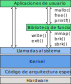
\includegraphics[scale=0.65]{img/library.pdf}}
    \end{center}
    \end{textblock}
\end{frame}

% https://en.wikipedia.org/wiki/C\_POSIX\_library
% https://en.wikipedia.org/wiki/C\_standard\_library

\begin{frame}[fragile]{Llamadas al Sistema Operativo: ejemplos}
    \begin{textblock}{75}(10,13)
    \textcolor{verdeuca}{Administración de archivos}
    \begin{itemize} \setlength\itemsep{0cm}
    \item \footnotesize Crear y borrar: \texttt{create} y \texttt{delete}.
    \item \footnotesize Abrir, cerrar: \texttt{open} y \texttt{close}.
    \item \footnotesize Leer, escribir y reposicionar: \texttt{read}, \texttt{write} y \texttt{lseek}.
    \end{itemize}
    \textcolor{verdeuca}{Administración de dispositivos}
    \begin{itemize} \setlength\itemsep{0cm}
    \item \footnotesize Solicitar y liberar: \texttt{open} y \texttt{close}.
    \item \footnotesize Leer, escribir y reposicionar: \texttt{read}, \texttt{write} y \texttt{lseek}.
    \end{itemize}
    \textcolor{verdeuca}{Control de ejecución}
    \begin{itemize} \setlength\itemsep{0cm}
    \item \footnotesize Terminar ejecución: \texttt{exit}.
    \item \footnotesize Cargar y ejecutar: \texttt{fork} y \texttt{exec}.
    \item \footnotesize Asignar y liberar memoria: \texttt{brk}, \texttt{sbrk} y \texttt{mmap}.
    \end{itemize}
    \textcolor{verdeuca}{Comunicación y sincronización}
    \begin{itemize} \setlength\itemsep{0cm}
    \item \footnotesize Notificación de eventos y espera entre procesos: \texttt{signal} y \texttt{wait}.
    \end{itemize}
    \textcolor{verdeuca}{Información del sistema}
    \begin{itemize} \setlength\itemsep{0cm}
    \item \footnotesize Fecha y hora: \texttt{date} y \texttt{time}.
    \end{itemize}
    \end{textblock}
    \begin{textblock}{65}(85,12)
    \begin{tcolorbox}[size=small,width=\textwidth,sharp corners,title={\footnotesize Ejemplo}]
    \footnotesize
    En un procesador \texttt{Intel} \texttt{x86} la forma de llamar a la syscall \texttt{exit} es:
    \begin{tcolorbox}[left skip=2.2cm,size=fbox,colback={verdeuca!30},width=2cm,sharp corners,title={}]
    \verb|...|\\
    \verb|mov eax, 1|\\
    \verb|mov ebx, 0|\\
    \verb|int 0x80|
    \end{tcolorbox}
    \textcolor{naranjauca}{\textbf{\texttt{eax}}} indica el múmero del servicio (\texttt{exit}).\\
    \textcolor{naranjauca}{\textbf{\texttt{ebx}}} el código de finalización del programa.\\
    Con esta operación terminamos la ejecución del programa.\\ \\
    \end{tcolorbox}
    \small
    \textcolor{gray}{Notar que los parámetros se pasan por registro\\
    y la instrucción \texttt{int} cambia el nivel de privilegio para acceder al sistema.}
    \end{textblock}
\end{frame}

\begin{frame}[fragile]{Llamadas al Sistema Operativo: ejemplos (\emph{buffer})}
    \begin{textblock}{60}(5,13) \uncover<1->{\includegraphics[scale=0.65]{img/llamado_libc-layer1.pdf}} \end{textblock}
    \begin{textblock}{60}(5,13) \uncover<2->{\includegraphics[scale=0.65]{img/llamado_libc-layer2.pdf}} \end{textblock}
    \begin{textblock}{60}(5,13) \uncover<3->{\includegraphics[scale=0.65]{img/llamado_libc-layer3.pdf}} \end{textblock}
    \begin{textblock}{60}(5,13) \uncover<4->{\includegraphics[scale=0.65]{img/llamado_libc-layer4.pdf}} \end{textblock}
    \begin{textblock}{60}(5,13) \uncover<5->{\includegraphics[scale=0.65]{img/llamado_libc-layer5.pdf}} \end{textblock}
    \begin{textblock}{60}(5,13) \uncover<6->{\includegraphics[scale=0.65]{img/llamado_libc-layer6.pdf}} \end{textblock}
    \begin{textblock}{60}(5,13) \uncover<7->{\includegraphics[scale=0.65]{img/llamado_libc-layer7.pdf}} \end{textblock}
    \begin{textblock}{60}(5,13) \uncover<7->{\includegraphics[scale=0.65]{img/llamado_libc-layer8.pdf}} \end{textblock}
    \begin{textblock}{60}(92,8)
    \begin{enumerate}
    \setlength\itemsep{0.4cm}
     \item<2-> La aplicación llama a \texttt{printf}.
     \item<3-> La función \texttt{printf} es parte de la \texttt{libc} y realizar el llamado al sistema \texttt{write}.
     \item<4-> El SO. resuelve el llamado. 
     \item<5-> El texto a imprimir se almacena en un \emph{buffer} dentro del SO.
     \item<6-> El SO. retorna el control a la aplicación (o a otra aplicación).
     \item<7-> El SO. resuelve las operaciones de entrada/salida escribiendo en la plantalla. 
    \end{enumerate}
    \end{textblock}
\end{frame}

\begin{frame}{Estructura del \emph{kernel}}
    El \emph{kernel} es el \textbf{núcleo} del Sistema Operativo.
    Contiene el código más básico de soporte para la admistración del Hardware y recursos del sistema.\\
    \medskip
    \textcolor{gray}{Usualmente está implementado en un lenguaje de programación como C o C++.\\
    Requiriendo además algunas líneas de \texttt{ASM} dependientes de la arquitectura destino.}\\
    \bigskip
    \begin{center}
    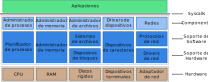
\includegraphics[scale=0.6]{img/kernel_architecture.pdf}
    \end{center}
\end{frame}

\begin{frame}{Estructura del \emph{kernel}}
    \begin{textblock}{78}(5,13)
    \only<1->{
    \small \textcolor{verdeuca}{Diseño Monolítico} \vspace{-0.2cm}
    \begin{itemize} \setlength\itemsep{-0.1cm}
    \item[] \scriptsize Todo el código puede \textbf{acceder} a los recursos y estructuras de datos del sistema.
    \item[] \scriptsize \textcolor{gray}{Pro:} Favorece la eficiencia.
    \item[] \scriptsize \textcolor{gray}{Contra:} Complejiza la mantenibilidad, extensibilidad y la corrección de errores.
    \end{itemize}
    }
    \only<2->{
    \small \textcolor{verdeuca}{Diseño \emph{Microkernel}} \vspace{-0.2cm}
    \begin{itemize} \setlength\itemsep{-0.1cm}
    \item[] \scriptsize Implementa un \textbf{conjunto mínimo} de funciones esenciales.\\
          El resto son programas de usuario que llaman a servicios.
    \item[] \scriptsize \textcolor{gray}{Pro:} Favorece la portabilidad y la extensibilidad.
    \item[] \scriptsize \textcolor{gray}{Contra:} Es menos eficiente, porque realiza muchas más \emph{syscalls}.
    \end{itemize}
    }
    \only<3->{
    \small \textcolor{verdeuca}{Diseño Modular} \vspace{-0.2cm}
    \begin{itemize} \setlength\itemsep{-0.1cm}
    \item[] \scriptsize Cuenta con un módulo principal de funciones básicas y otros módulos que implementan funciones específicas que pueden interactuar entre sí.
    Permite cargar nuevos módulos, agregando funcionalidades al sistema.
    \item[] \scriptsize \textcolor{gray}{Pro:} Favorece la eficiencia, la mantenibilidad, extensibilidad y la corrección de errores.
    \end{itemize}
    }
    \only<3->{
    \vspace{-0.2cm}
    \begin{center}
    \small \textcolor{naranjauca}{Estrategia actual de diseño de kernels.}
    \end{center}
    }
    \end{textblock}
%     \begin{textblock}{60}(155,27) \rotatebox{90}{\textcolor{naranjauca}{\textbf{Tipos de diseños de kernels}}}\end{textblock}
%     \begin{textblock}{60}(150,14) \rotatebox{90}{\textcolor{verdeuca}{\scriptsize Diseño Monolítico}} \end{textblock}
%     \begin{textblock}{60}(150,58) \rotatebox{90}{\textcolor{verdeuca}{\scriptsize Diseño \emph{Microkernel}}} \end{textblock}
    \begin{textblock}{60}(95,4)  \only<1->{\includegraphics[scale=0.45]{img/monolitico_microkernel-layer1.pdf} } \end{textblock}
    \begin{textblock}{60}(95,48) \only<2->{\includegraphics[scale=0.45]{img/monolitico_microkernel-layer2.pdf} } \end{textblock}
    \begin{textblock}{60}(115,19) \only<1->{\centering \textcolor{verdeuca}{\small Diseño\\ Monolítico} } \end{textblock}
    \begin{textblock}{60}(115,63) \only<2->{\centering \textcolor{verdeuca}{\small Diseño\\ \emph{Microkernel}} } \end{textblock}
\end{frame}

\begin{frame}{Inicialización del Sistema Operativo}
    \begin{textblock}{140}(90,1) \only<4->{ \includegraphics[scale=0.35]{img/inicio-layer1.pdf} } \end{textblock}
    \begin{textblock}{140}(90,1) \only<5->{ \includegraphics[scale=0.35]{img/inicio-layer2.pdf} } \end{textblock}
    \begin{textblock}{140}(90,1) \only<6->{ \includegraphics[scale=0.35]{img/inicio-layer3.pdf} } \end{textblock}
    \begin{textblock}{140}(90,1) \only<7->{ \includegraphics[scale=0.35]{img/inicio-layer4.pdf} } \end{textblock}
    \begin{textblock}{140}(90,1) \only<8->{ \includegraphics[scale=0.35]{img/inicio-layer5.pdf} } \end{textblock}
    \begin{textblock}{70}(10,15)
    \small
    Existen varias formas de inicializar un sistema.\\
    \medskip
    \uncover<2->{
    Cada una depende del \textbf{Sistema Operativo a cargar} y del \textbf{soporte en hardware} con el que se cuente.\\
    }
    \medskip
    \uncover<3->{
    \small
    \textcolor{verdeuca}{La forma \textbf{Legacy} o \emph{BIOS Boot} fue la utilizada por las primeras IBM PC compatibles.\\
    \medskip
    \scriptsize
    Esta forma es \textbf{limitada} e \textbf{insegura}, ya que no garantiza la integridad el sistema, ni permite particiones grandes.\\}
    }
    \bigskip
    \uncover<4->{
    \small
    La forma actual para inicializar un sistema es \textbf{UEFI} \textit{(Unified Extensible Firmware Interface)}.\\
    \medskip
    \scriptsize
    Es una interfaz desarrollada por Intel en 2002, con una arquitectura modular que permite disponer de todos los recursos del sistema.
    Evitando las limitaciones de utilizar el MBR, y permitiendo utilizar discos con particiones grandes.\\
    Además de contar con soporte para encriptación y chequeo de integridad.
    }
    \end{textblock}
\end{frame}

\begin{frame}[fragile,c]
    \frametitle{Bibliografía}
    \begin{itemize}
        \setlength\itemsep{0.5cm}
        \item[-] \small Silberschatz, ``Fundamentos de Sistemas Operativos'', 7ma Edición, 2006.\\
        \vspace{0.4cm}
        \begin{itemize}
            \setlength\itemsep{0.5cm}
            \item \textbf{Capítulo 1 - Introducción}
            \begin{itemize}
                \setlength\itemsep{0.2cm}
                \item 1.1 ¿Qué hace un sistema operativo? - Páginas 3-6
                \item 1.4 Estructura de un sistema operativo - Páginas 14-16
                \item 1.5 Operaciones del sistema operativo - Páginas 16-18
            \end{itemize}
            \item \textbf{Capítulo 2 - Estructura de sistemas operativos}\\ (salvo sección 2.8 Máquinas virtuales), páginas 35-57 y 63-64
        \end{itemize}
    \end{itemize}
\end{frame}

\begin{frame}[plain]
    \begin{center}
    \vspace{2cm}
    \huge ¡Gracias!\\
    \vspace{2cm}
    \normalsize Recuerden leer los comentarios adjuntos\\ en cada clase por aclaraciones.
    \end{center}
\end{frame}

\end{document}
